\section{Extended threshold analysis}
\label{sec:s-threshold}

This section extends Section~\ref{M-sec:theory} of the main text beyond $N=3$, with pair-dependent judges, correlated wrong answers, a large-$N$ lower bound and the cost term.

\begin{lemma}[Monotone coupling]
\label{lem:monotone}
For every $N$ and every $\rho$, the probability that the Copeland selector
returns a correct candidate is nondecreasing in each $q_{ij}$.
\end{lemma}

\begin{corollary}[Pair-dependent judges]
\label{cor:pairdep}
Let $q^{*}(p,N,\rho)$ be the smallest uniform $q$ at which the selector ties
voting. A judge with $q_{ij}\ge q^{*}$ for all mixed pairs is at least as accurate
as voting; one with $q_{ij}\le q^{*}$ for all mixed pairs is at most as accurate.
\end{corollary}

Table~\ref{tab:threshold-n} gives $q^{*}$ computed exactly for $N=3,\dots,7$
(the $N=3$, $\rho=0$ column reproduces Table~\ref{M-tab:threshold}). Two things stand
out. With distinct wrong answers the threshold \emph{rises} with $N$: at
$p=0.8$ it goes from $0.804$ to $0.935$, and Proposition~\ref{prop:lower} below shows that this is not an artefact of small $N$: the threshold cannot fall back towards chance as $N$ grows. With correlated wrong answers ($\rho=0.5$) voting is weaker
and the threshold is lower, about $0.82$ at $p=0.8$ for $N\ge4$. The
direction of the relaxation is therefore the one a reader would expect, but its
size is large enough that the realistic threshold is far from $\tfrac12$.
For GPQA Diamond, whose wrong answers are heavily correlated, this lowers the
threshold from $0.787$ to $0.714$
(Table~\ref{M-tab:threshold-emp-gen}); the measured $\hat q=0.536$ remains far below it.
We checked the exact enumeration against an independent Monte Carlo
simulation with common random numbers (Table~\ref{tab:threshold-valid}; all
four configurations agree within sampling error) and checked
Corollary~\ref{cor:pairdep} on random pair-dependent judges: in
\PairDepInside{} of \PairDepTrials{} random $N=5$ instances the accuracy gap lies
between the gaps at $q_{\min}$ and $q_{\max}$.

\begin{table}[htbp]
\centering
\caption{Exact break-even pairwise accuracy $q^{*}(p,N,\rho)$ for the Copeland
selector against plurality voting, with per-candidate accuracy $p$ and
wrong-answer correlation $\rho$.}
\label{tab:threshold-n}
\small
\begin{tabular}{rrrrr}
\toprule
 & \multicolumn{2}{c}{$\rho=0$} & \multicolumn{2}{c}{$\rho=0.5$} \\
\cmidrule(lr){2-3}\cmidrule(lr){4-5}
$N$ & $p=0.5$ & $p=0.8$ & $p=0.5$ & $p=0.8$ \\
\midrule
\ThresholdNRows
\ThresholdNSevenRow
\bottomrule
\end{tabular}
\end{table}

\begin{table}[htbp]
\centering
\caption{Exact accuracy gap (Copeland minus plurality, percentage points) against a
200{,}000-draw Monte Carlo estimate with its standard error.}
\label{tab:threshold-valid}
\small
\begin{tabular}{rrrrrr}
\toprule
$N$ & $p$ & $\rho$ & $q$ & Exact & Monte Carlo \\
\midrule
\ThresholdValidationRows
\bottomrule
\end{tabular}
\end{table}

\paragraph{Why the threshold keeps rising: a large-$N$ lower bound}
With distinct wrong answers plurality's error has a closed form. It is correct
whenever at least two candidates are correct, and when exactly one is correct all $N$ answers
differ and it is chosen with probability $1/N$, so
\begin{equation}
\mathrm{err}_{V}(N)=(1-p)^{N}+(N-1)\,p\,(1-p)^{N-1},
\label{eq:vote-err}
\end{equation}
which decays at rate $-\ln(1-p)$ per candidate. A pairwise-Copeland selector
that errs on the event ``a wrong candidate beats a sizeable block of correct ones''
decays more slowly unless $q$ is large. Write
$\mathrm{KL}(\eta\Vert p)=\eta\ln\frac{\eta}{p}+(1-\eta)\ln\frac{1-\eta}{1-p}$ and
\[
\Lambda(p,q)\;=\;\inf_{\eta>1-\frac{1}{2q}}\Bigl[\mathrm{KL}(\eta\Vert p)+\eta\ln\tfrac{1}{1-q}\Bigr].
\]

\begin{proposition}[Large-$N$ lower bound]
\label{prop:lower}
Let wrong answers be distinct ($\rho=0$) and the judge uniform with $q>\tfrac12$. If
$\Lambda(p,q)<-\ln(1-p)$, there is $N_0$ such that for all $N\ge N_0$ the Copeland selector is strictly
less accurate than plurality. Consequently $\liminf_{N\to\infty}q^{*}(p,N)\ge q_{\Lambda}(p)$, where
$q_{\Lambda}(p)$ is the unique root of $\Lambda(p,q)=-\ln(1-p)$.
\end{proposition}

Table~\ref{tab:threshold-lambda} lists $q_{\Lambda}(p)$ next to the exact $N=6$ thresholds:
the exact values sit just below the limiting lower bound for $p\ge0.6$ and just above it at $p=0.5$,
as a sequence rising to (at least) $q_{\Lambda}$ would. We do not prove that the limit equals $q_{\Lambda}$; the
proposition is a lower bound, obtained by exhibiting one specific way in which Copeland errs.

\begin{table}[htbp]
\centering
\caption{Plurality's error decay rate $-\ln(1-p)$, the large-$N$ lower bound $q_{\Lambda}(p)$ on
$\liminf_N q^{*}(p,N)$ (Proposition~\ref{prop:lower}), and the exact $q^{*}(p,6)$ ($\rho=0$).}
\label{tab:threshold-lambda}
\small
\begin{tabular}{rrrr}
\toprule
$p$ & $-\ln(1-p)$ & $q_{\Lambda}(p)$ & $q^{*}(p,6)$ \\
\midrule
\ThresholdLambdaRows
\bottomrule
\end{tabular}
\end{table}

\paragraph{Structure of the wrong answers beyond a single attractor}
The attractor model with parameter $\rho$ is one way to correlate wrong answers. We also
drew each wrong answer uniformly from $D$ wrong values ($D=1$: all wrong answers coincide;
$D=3$: the three distractors of a four-option question; $D=\infty$: all distinct).
Table~\ref{tab:threshold-D} shows that the threshold is monotone in the structure: the fewer distinct wrong values, the
weaker plurality and the lower the threshold, down to $q^{*}=\tfrac12$ when all wrong answers coincide and the
pool is small ($N=4$, $p=0.5$). For the four-option GPQA questions ($D=3$) the threshold is $0.64$--$0.80$ at
$N=4,5$, consistent with the attractor-model estimate for GPQA in Table~\ref{M-tab:threshold-emp-gen}.

\begin{table}[htbp]
\centering
\caption{Exact $q^{*}$ when each wrong answer is uniform over $D$ wrong values.}
\label{tab:threshold-D}
\small
\begin{tabular}{rrrrr}
\toprule
 & \multicolumn{2}{c}{$N=4$} & \multicolumn{2}{c}{$N=5$} \\
\cmidrule(lr){2-3}\cmidrule(lr){4-5}
$D$ & $p=0.5$ & $p=0.8$ & $p=0.5$ & $p=0.8$ \\
\midrule
\ThresholdDRows
\bottomrule
\end{tabular}
\end{table}

\paragraph{The cost term} The results above use the quality term alone, the case most
favourable to the judge. If the cost (length) of a candidate is independent of its
correctness, adding it can only move the selector towards the shortest-candidate rule, whose accuracy is
exactly $p$, the accuracy of a random pick; Table~\ref{tab:threshold-cost} shows by simulation how accuracy
falls from the judge-only value to $p$ as the cost weight $\lambda$ (relative to the Copeland score
scaled to $[0,1]$) grows. In our data lengths are not independent of correctness (shortest-candidate accuracy
differs from the random-pick accuracy, Table~\ref{tab:baselines}), so the empirical effect of the cost term is a
property of the data, which Section~\ref{M-sec:cost-diagnosis} measures directly.

\begin{table}[htbp]
\centering
\caption{Simulated accuracy (\%) of selection by Copeland score minus $\lambda\times$ an independent random
length, $N=3$, $p=0.8$ (plurality voting: 92.8\%; random pick: 80.0\%), 100{,}000 draws.}
\label{tab:threshold-cost}
\small
\begin{tabular}{lrr}
\toprule
$\lambda$ & $q=0.6$ & $q=0.9$ \\
\midrule
\ThresholdCostRows
\bottomrule
\end{tabular}
\end{table}

\paragraph{Large $N$: a regime split, not a threshold} For large $N$ the
break-even accuracy is no longer informative, because both selectors approach
perfect accuracy whenever correct answers form a plurality; the difference
then lives in exponentially small error rates, which a threshold at fixed
accuracy does not capture. What can be said rigorously is a consistency result.

\begin{proposition}[Large-$N$ regimes]
\label{prop:regimes}
Let candidates be independent with correct-answer probability $p>0$, wrong answers taking finitely many values, and let $m$ be the largest probability of any single wrong answer. (i) Plurality voting
is correct with probability tending to $1$ if $p>m$ and to $0$ if $p<m$. (ii) If
$q_{ij}\ge q_{\min}>\tfrac12$ for all mixed pairs, the Copeland selector is
correct with probability at least $1-(1-p)^N-2N^{2}e^{-(q_{\min}-1/2)^{2}N/2}\to1$,
whatever $m$.
\end{proposition}

So a judge that is better than chance can rescue a generator pool in which the
single most popular answer is wrong ($p<m$), where plurality voting fails with
certainty, but it cannot be expected to improve a pool in which the right answer
already leads. This is the pairwise-judge analogue of the dichotomy established
for reward-model best-of-$N$ and majority voting by \citet{di2025bom}, and we
claim consistency with it, not novelty: the contribution here is the exact
finite-$N$ thresholds above and their confrontation with the measured $\hat q$.
Our benchmark pools are in the right-majority regime (the shipped Nemotron generator is correct on 77--99\% of candidates, floor column of Table~\ref{M-tab:recovery}),
which is why the judge cannot help.


\section{Proofs for the extended threshold analysis}
\label{sec:s-proofs}

\label{app:proof2}

\emph{Lemma~\ref{lem:monotone}.} Fix a mixed pair $(c,w)$ with $c$ correct and $w$ wrong and
condition on all other comparison outcomes; the outcome of $(c,w)$ is a
Bernoulli($q_{cw}$) variable that is the only one depending on $q_{cw}$, so it
suffices to show that changing it from ``$w$ wins'' to ``$c$ wins'' cannot lower the
probability that the selected candidate is correct. The change raises $c$'s score by one and lowers $w$'s by one.
Let $T$ be the set of top scorers before and $T'$ after, and let the selected candidate be uniform on the top set, so the success
probability is the share of correct candidates in it. If $c\in T$, then $T'=\{c\}$, which is correct. If
$c\notin T$ and $w\notin T$, then $T'=T$ or $T'=T\cup\{c\}$; adding a correct candidate cannot lower a
share that is at most one. If $w\in T$ and $|T|>1$, then $T'$ removes $w$ and possibly adds $c$, which
cannot lower the share. If $w$ is the unique top scorer, the share before is $0$. In every case the share does not decrease.
Averaging over the other outcomes gives the claim, and Corollary~\ref{cor:pairdep} follows by comparing with the uniform judges at $q_{\min}$
and $q_{\max}$ (voting does not depend on the judge).

\emph{Proposition~\ref{prop:regimes}.} (i) The count of the correct answer is Binomial$(N,p)$ and that of each wrong answer is Binomial$(N,\cdot)$ with success probability at most $m$, the largest attaining $m$; by Hoeffding's inequality and a union bound over the finitely many answers, the correct answer is the unique plurality with probability tending to one if $p>m$, and is beaten by the most popular wrong answer with probability tending to one if $p<m$. (ii) Condition on the set of correct candidates, of size $k_c\ge1$ (probability $1-(1-p)^N$), and let
$k_w=N-k_c$. A correct candidate's score is a sum of $N-1$ independent comparisons with mean at least
$q_{\min}k_w+\tfrac12(k_c-1)$; a wrong candidate's has mean at most $(1-q_{\min})k_c+\tfrac12(k_w-1)$; the
difference is at least $(q_{\min}-\tfrac12)N$. By Hoeffding's inequality each score is within
$t=(q_{\min}-\tfrac12)N/2$ of its mean with probability at least
$1-2\exp(-2t^2/(N-1))\ge1-2\exp(-(q_{\min}-\tfrac12)^2N/2)$. A union bound over the $N$ candidates gives
the stated probability that every correct candidate outscores every wrong one, in which case the selected
candidate is correct. \qed

\emph{Equation~\eqref{eq:vote-err}.} With distinct wrong answers the plurality is the correct answer exactly when
at least two candidates are correct (its count then exceeds every wrong count, which is one); with one correct candidate
all $N$ answers are tied and the correct one is chosen with probability $1/N$; with none it cannot be chosen. Hence
$\mathrm{err}_V=(1-p)^N+Np(1-p)^{N-1}(1-1/N)$.

\emph{Proposition~\ref{prop:lower}.} Fix $q>\tfrac12$ and $\eta\in(1-\tfrac1{2q},1)$ and let $K=\lceil\eta N\rceil$. Consider the event $E$ that
exactly $K$ candidates are correct and a designated wrong candidate $w$ beats all of them (probability
$\binom NK p^K(1-p)^{N-K}(1-q)^K\ge \frac{1}{N+1}e^{-N\,\mathrm{KL}(K/N\Vert p)}(1-q)^K$). Conditionally on $E$, $w$'s score is $K+\mathrm{Bin}(N-K-1,\tfrac12)$,
with mean $(N+K-1)/2$; a correct candidate's score has mean at most $q(N-K-1)+(K-1)/2+0$ (it has already lost to $w$), and another wrong
candidate's has mean $(1-q)K+(N-K-1)/2$. The gaps are $N(\tfrac12-q(1-\eta))+O(1)$ and $qK$, linear in $N$ and positive because
$\eta>1-\tfrac1{2q}$. By Hoeffding's inequality and a union bound over the $N$ candidates, $w$ is the unique top scorer with conditional probability
$1-O(N e^{-cN})$, so the Copeland selector errs on $E$ with probability at least $\tfrac12$ for large $N$. Therefore
$\mathrm{err}_C\ge\frac{1}{2(N+1)}e^{-N[\mathrm{KL}(\eta\Vert p)+\eta\ln\frac1{1-q}+o(1)]}$. If $\Lambda(p,q)<-\ln(1-p)$ choose $\eta$
with bracket below $-\ln(1-p)$; since $\mathrm{err}_V\le N(1-p)^{N-1}$ by Equation~\eqref{eq:vote-err}, $\mathrm{err}_C>\mathrm{err}_V$ for all large $N$.
For the consequence: $\Lambda(p,q)$ is continuous and strictly increasing in $q$ (it equals an infimum of functions
increasing in $q$ over a set that shrinks with $q$), lies below $-\ln(1-p)$ for $q$ slightly above $\tfrac12$ (the derivative of $\mathrm{KL}(\eta\Vert p)$ is $-\infty$ at $\eta=0$) and
diverges as $q\uparrow1$ (it is at least $\tfrac12\ln\frac1{1-q}$), so $q_\Lambda(p)$ exists and is unique. For any $\epsilon>0$ the accuracy gap at $q_\Lambda-\epsilon$ is negative for large
$N$, and by Lemma~\ref{lem:monotone} it is nonincreasing as $q$ decreases, so it is negative for every $q\le q_\Lambda-\epsilon$. Hence
$q^{*}(p,N)>q_\Lambda-\epsilon$ for large $N$. \qed


\section{Additional selectors}
\label{sec:baselines}

Table~\ref{tab:baselines} compares OR-Select's competitors beyond
Section~\ref{M-sec:accuracy-results}. Judge-free selectors (shortest and
longest candidate, and minimum-Bayes-risk selection with token-set Jaccard
similarity) run on every graded problem; judge-based selectors are replayed on
the problems whose judge outputs were stored (pointwise confidence argmax,
a vote weighted by the scorer's confidence, a knockout tournament over the
pairwise matrix, and a Bradley--Terry fit). Each is paired with
self-consistency on the same problems; the parenthesis in each accuracy cell
is the self-consistency accuracy on those problems.

No selector beats plurality voting in either condition. The judge-free
minimum-Bayes-risk selector, which only measures how much a candidate
resembles the others, stays within a few problems of voting in both
conditions, and so does the confidence-weighted vote, which is itself a
variant of voting. The selectors that act on the judge's pairwise or pointwise
output choose worse than voting in heterogeneous pools, as OR-Select does,
and the trivial length rules (shortest, longest) are worse still. The
common thread is the same as in Section~\ref{M-sec:cost-diagnosis}: whatever
signal the judge adds is not about correctness.

\begin{table}[htbp]
\centering
\caption{Additional selectors, paired with self-consistency (SC) on the same
graded problems. For each condition: problems $n$, accuracy \% (SC accuracy
\% on the same problems), problems where the selector is right and SC wrong
over the reverse, and the exact McNemar $p$. $^\dagger$: needs the stored
judge outputs, so $n$ is the replayable subset.}
\label{tab:baselines}
\small\setlength{\tabcolsep}{4pt}
\resizebox{\textwidth}{!}{%
\begin{tabular}{lrrrrrrrr}
\toprule
 & \multicolumn{4}{c}{Homogeneous} & \multicolumn{4}{c}{Heterogeneous} \\
\cmidrule(lr){2-5}\cmidrule(lr){6-9}
Selector & $n$ & Acc. (SC) & W/L & $p$ & $n$ & Acc. (SC) & W/L & $p$ \\
\midrule
\BaselineTableRows
\bottomrule
\end{tabular}}
\end{table}


\section{Coverage and higher-cap second pass: tables}
\label{sec:s-coverage}

\begin{table}[htbp]
\centering
\caption{Coverage by track. Truncated: no valid answer after resampling
because generation hit the output cap. Other: failed for another reason.
Untried: not attempted. With Laguna: graded heterogeneous
problems that still contain Laguna-S candidates.}
\label{tab:coverage}
\small\setlength{\tabcolsep}{4pt}
\resizebox{\textwidth}{!}{%
\begin{tabular}{lrrrrrr}
\toprule
Track & Total & Graded & Truncated & Other & Untried & With Laguna \\
\midrule
\CoverageTableRows
\bottomrule
\end{tabular}}
\end{table}

\begin{table}[htbp]
\centering
\caption{Effect of the flagged second pass. Main protocol: problems that
completed under the 32{,}768-token cap. Rescued: problems completed only
under the higher cap. Final: all graded problems.}
\label{tab:extended}
\small\setlength{\tabcolsep}{4pt}
\resizebox{\textwidth}{!}{%
\begin{tabular}{lrrrrrr}
\toprule
Track & Main n & Main OR & Main SC & Rescued & Final OR & Final SC \\
\midrule
\ExtendedTableRows
\bottomrule
\end{tabular}}
\end{table}


\section{Pilot illustration: open-ended queries}
\label{sec:pilot}

Three open-ended queries ($N=5$ each, no ground truth) were run in an
earlier pilot to check that the pipeline behaves sensibly where
self-consistency has nothing to vote on. Across the 15 candidates, none was
byte-identical to another, so self-consistency resorted to an arbitrary
tie-break on every query, and OR-Select differed from both baselines on all
three (score margins 0.088, 0.446 and a near-tie of 0.003). With three
queries and no ground truth this is an illustration, not evidence about
quality. Two pilot ablations on the same candidate sets (setting $w_4=0$;
forward-only judging) changed 0 and 2 of the 3 winners respectively: the
self-consistency term was inert because no candidate set clustered, and
bidirectional judging mattered in two of three cases, consistent with
position bias being a first-order judge failure mode
\citep{zheng2023judging,tang2024permutation,wang2023notfair}. Three
instances cannot characterize when the directions disagree.


\section{A concrete non-determinism finding}
\label{sec:seed-finding}

In an earlier pilot run on a different provider and model, three candidates
had byte-identical text. By construction every pairwise weight among
identical text must be $0.5$, since the forward and backward judge calls
are the same prompt and $(v+(1-v))/2=0.5$. The observed quality scores
were $0.375$, $0.50$ and $0.625$, direct evidence that the provider's \texttt{seed} parameter was not reliably honored in that run,
in line with systematic run-to-run variation reported for nominally deterministic
settings \citep{atil2024nondeterminism}. This is a
single observation; the exact-match short-circuit
(Section~\ref{M-sec:pipeline}) removes this failure mode for identical text
but not for different texts that receive unstable scores, which remains
open.


\section{Retry independence and extraction fallbacks}
\label{sec:validity-fix}

Each validity-retry draws with a freshly varied seed, so a persistently
invalid slot gets three independent samples rather than three repeats of
what a seed-honoring backend already returned. Extraction accepts more than
one marker: GPQA also recognizes a prose ``the answer is X'' pattern
alongside \texttt{ANSWER:\ X} and \texttt{\textbackslash boxed\{X\}},
because its answer space is four letters; MATH's open-ended
\texttt{\textbackslash boxed\{\}} extraction has no prose fallback, since a
wrong guess there would convert an honest ``ungraded'' problem into a
confidently incorrect one. This asymmetry is a design choice.


\section{Worked example and positional-bias figure}
\label{sec:s-worked}

Table~\ref{tab:worked-example} and
Figure~\ref{fig:worked-example} decompose Equation~\eqref{M-eq:selection-obj}
for one real open-ended run ($N=5$, no exact-text duplicates).
$\text{quality}_i$ is recovered by inverting the saved
$\text{score}_i$ against the known confidence, cost and consistency, and the
recovered argmax is checked by script against the saved winner.

\begin{table}[htbp]
\centering
\caption{Component scores for one real open-ended run (winner marked
$^\ast$). $\text{quality}_i$ is recovered by inversion, not stored directly.}
\label{tab:worked-example}
\begin{tabular}{lrrrrr}
\toprule
Candidate & $\text{quality}_i$ & $\text{confidence}_i$ & $\text{consistency}_i$ & $\text{cost}_i$ & $\text{score}_i$ \\
\midrule
\WorkedExampleTableRows
\bottomrule
\end{tabular}
\end{table}

\begin{figure}[htbp]
\centering
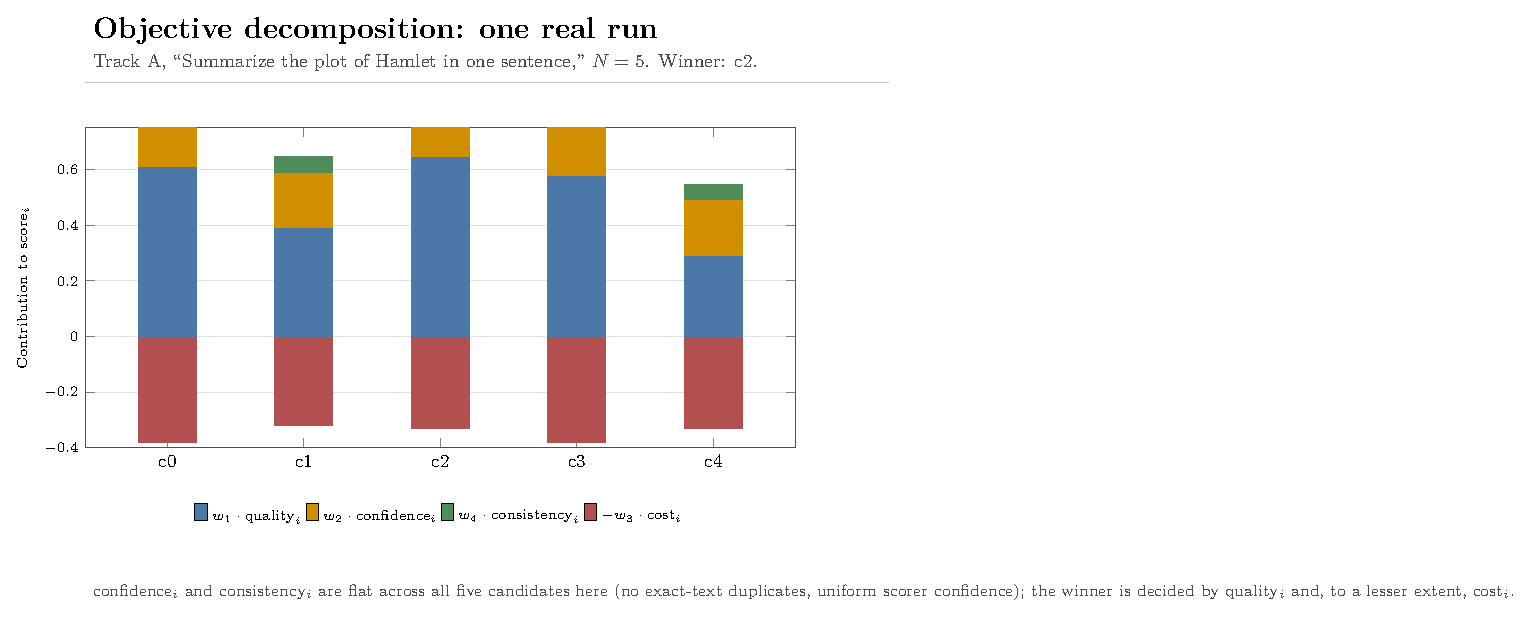
\includegraphics[width=0.85\textwidth]{Figure_3_WorkedExample.pdf}
\caption{The same run as Table~\ref{tab:worked-example}, as stacked weighted
contributions to $\text{score}_i$. Confidence and consistency are constant
across candidates here (no duplicates; uniform scorer confidence), so the
ranking is decided by quality and cost. These candidates are one-sentence
summaries; on multi-hundred-word reasoning outputs the cost term is far
larger relative to quality (Section~\ref{M-sec:cost-diagnosis}).}
\label{fig:worked-example}
\end{figure}


\begin{figure}[htbp]
\centering
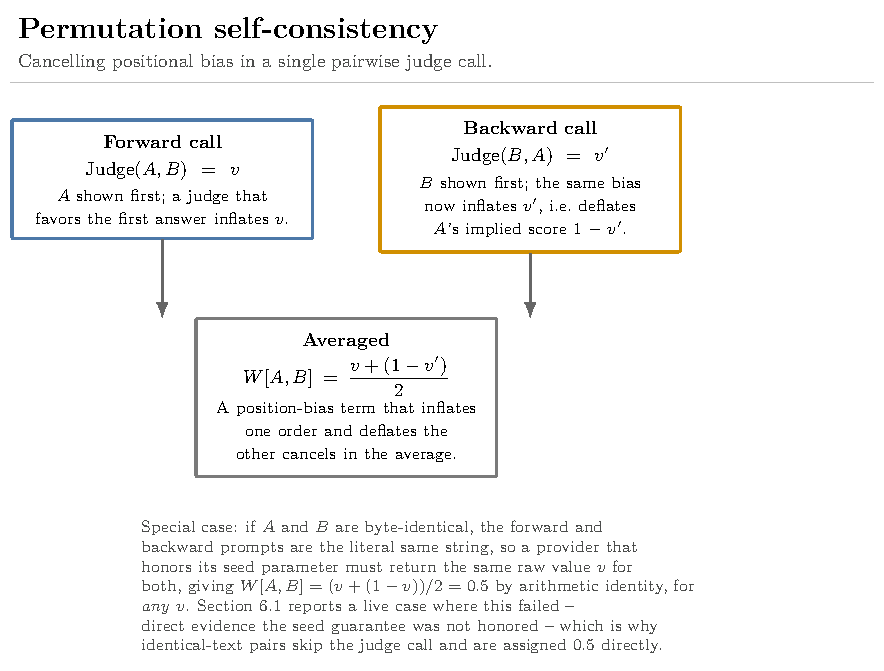
\includegraphics[width=0.85\textwidth]{Figure_2_BiasCancellation.pdf}
\caption{Permutation self-consistency cancels positional bias by averaging
the forward and (complement-transformed) backward judge calls for each
pair. Byte-identical candidates force $W=0.5$ by arithmetic identity,
independent of the judge's output.}
\label{fig:bias-cancel}
\end{figure}

